\documentclass[conference]{IEEEtran}
% \IEEEoverridecommandlockouts % só necessário se houver \thanks de financiamento

\usepackage[utf8]{inputenc}
\usepackage[T1]{fontenc}
\usepackage[brazilian]{babel}
\usepackage{cite}
\usepackage{amsmath,amssymb,amsfonts}
\usepackage{graphicx}
\graphicspath{{figuras/}}
\usepackage{textcomp}
\usepackage{xcolor}
\usepackage{listings}
\usepackage{booktabs}
\usepackage{tikz}
\usetikzlibrary{arrows.meta,positioning}
\usepackage{url}

% ---------------------------------------------------------------
% Destaque de sintaxe para a linguagem Tupã
% ---------------------------------------------------------------
\lstdefinelanguage{Tupa}{
  morekeywords={dispositivo,ao,se,senao,inteiro,verdadeiro,falso,botao},
  morekeywords=[2]{nfc,led,ir,esperar,escrever},
  sensitive=true,
  morecomment=[l]{\#},
  morestring=[b]",
}
\lstset{
  basicstyle=\ttfamily\footnotesize,
  keywordstyle=\bfseries\color{orange!80!black},
  keywordstyle=[2]\color{teal!70!black},
  commentstyle=\itshape\color{gray},
  stringstyle=\color{red!60!black},
  numbers=left,
  numberstyle=\tiny\color{gray},
  numbersep=6pt,
  frame=single,
  rulecolor=\color{gray!40},
  breaklines=true,
  showstringspaces=false,
  tabsize=4,
  xleftmargin=1.5em,
  framexleftmargin=1.5em,
  captionpos=b,
  literate={á}{{\'a}}1 {é}{{\'e}}1 {í}{{\'i}}1 {ó}{{\'o}}1 {ú}{{\'u}}1
           {ã}{{\~a}}1 {õ}{{\~o}}1 {ç}{{\c{c}}}1 {â}{{\^a}}1 {ê}{{\^e}}1
}
\renewcommand{\lstlistingname}{Listagem}

\begin{document}

% ---------------------------------------------------------------
% Título (sem símbolos, caracteres especiais ou notas de rodapé)
% ---------------------------------------------------------------
\title{Tupã: Uma Linguagem de Domínio Específico em Português para Programação de Microcontroladores ESP32}

\author{
\IEEEauthorblockN{Michel Lutegar}
\IEEEauthorblockA{\textit{Engenharia de Computação} \\
\textit{IBMEC}\\
Rio de Janeiro, Brasil \\
email@aluno.ibmec.edu.br} % TODO: e-mail de Michel (so o Joao sabe)
\and
\IEEEauthorblockN{André Costa}
\IEEEauthorblockA{\textit{Engenharia de Computação} \\
\textit{IBMEC}\\
Rio de Janeiro, Brasil \\
email@aluno.ibmec.edu.br} % TODO: e-mail de Andre (so o Joao sabe)
\and
\IEEEauthorblockN{Felipe Dutrain} 
\IEEEauthorblockA{\textit{Engenharia de Computação} \\
\textit{IBMEC}\\
Rio de Janeiro, Brasil \\
202402011359@alunos.ibmec.edu.br}
\and
\IEEEauthorblockN{Guilherme Lopes}
\IEEEauthorblockA{\textit{Engenharia de Computação} \\
\textit{IBMEC}\\
Rio de Janeiro, Brasil \\
202401632473@aluno.ibmec.edu.br} % TODO: confirmar dominio do e-mail de Guilherme (aluno vs alunos; o de Felipe usa alunos)
}

\maketitle

% ---------------------------------------------------------------
% Resumo (sem símbolos, matemática ou notas de rodapé)
% ---------------------------------------------------------------
\begin{abstract}
Programar microcontroladores ainda exige domínio de C++, de bibliotecas
específicas e da configuração manual de pinos, o que representa uma barreira
significativa para iniciantes, estudantes e entusiastas de eletrônica. Este
artigo apresenta o Tupã, uma linguagem de domínio específico com sintaxe em
português e eventos de hardware como construções de primeira classe, voltada
para a placa ESP32. O compilador, implementado em Python, percorre as quatro
fases clássicas de compilação, análise léxica, análise sintática, análise
semântica e geração de código, e produz um programa Arduino em C++ destinado à compilação e à gravação na
placa pela Arduino CLI, etapa que ainda é manual. A análise semântica
verifica o uso correto dos módulos de hardware antes da gravação e emite
mensagens de erro didáticas em português. Em um exemplo de controle de acesso
por cartão NFC, um programa de 12 linhas de código em Tupã gera 100 linhas de
código C++, cerca de 8,3 vezes mais, sem que o usuário precise escrever inclusões de bibliotecas,
definições de pinos ou as funções de configuração e laço principal. Os
programas gerados compilam com a Arduino CLI, e um teste de bancada com
firmware escrito à mão validou o protótipo com ESP32-WROVER, leitor RC522 e
sensor infravermelho de obstáculo. O projeto encontra-se em desenvolvimento,
com as quatro fases do compilador implementadas e a gravação do código gerado
na placa ainda pendente.
\end{abstract}

\begin{IEEEkeywords}
compiladores, linguagem de domínio específico, sistemas embarcados, ESP32,
Arduino, ensino de programação
\end{IEEEkeywords}

% ===============================================================
\section{Introdução}
% ===============================================================
A popularização de placas de baixo custo, como Arduino e ESP32, aproximou
estudantes e entusiastas do desenvolvimento de sistemas embarcados. Ainda
assim, o caminho entre a ideia e o hardware funcionando costuma ser longo:
mesmo uma aplicação simples, como acender um LED quando um cartão válido é
aproximado de um leitor, exige incluir bibliotecas, definir pinos,
inicializar periféricos e organizar o código nas funções \texttt{setup()} e
\texttt{loop()} do ambiente Arduino. Para quem não domina C++, a configuração
do hardware frequentemente consome mais tempo do que a lógica da aplicação.

Somam-se a isso a barreira do idioma, já que palavras-chave, bibliotecas e
documentação estão majoritariamente em inglês, e o fato de que ferramentas
educacionais existentes ou dependem de hardware fechado, ou trabalham com
blocos visuais que não evoluem para uma linguagem textual.

Este trabalho propõe o \textit{Tupã}, uma linguagem de domínio específico
(DSL, do inglês \textit{domain-specific language}) com sintaxe em português,
cujo compilador traduz programas de alto nível para C++ compatível com o
ecossistema Arduino e executável no ESP32. A premissa central é que o usuário
descreva \emph{o que} o dispositivo deve fazer, e não \emph{como} o hardware
deve ser configurado, delegando ao compilador o trabalho de baixo nível.

As principais contribuições são:
\begin{itemize}
\item o projeto de uma linguagem textual em português com eventos de
hardware de primeira classe, como \texttt{ao botao(1) \{ \ldots\ \}};
\item um compilador completo, implementado em Python, que percorre as fases
de análise léxica, sintática e semântica e de geração de código;
\item uma análise semântica orientada ao hardware, que detecta erros antes
da gravação na placa e produz mensagens didáticas em português;
\item uma avaliação preliminar que compara o código escrito em Tupã com o
código C++ equivalente gerado.
\end{itemize}

O restante do artigo está organizado da seguinte forma: a Seção~\ref{sec:relacionados}
discute trabalhos relacionados; a Seção~\ref{sec:linguagem} descreve a
linguagem; a Seção~\ref{sec:compilador} detalha a arquitetura do compilador;
a Seção~\ref{sec:resultados} apresenta resultados preliminares; e a
Seção~\ref{sec:conclusao} conclui e aponta trabalhos futuros.

% ===============================================================
\section{Trabalhos Relacionados}\label{sec:relacionados}
% ===============================================================
O \textit{Arduino IDE} \cite{arduino} consolidou-se como a principal porta de
entrada para a programação de microcontroladores. Sua linguagem, um
subconjunto de C++ acompanhado de bibliotecas, é poderosa e madura, mas exige
do usuário conhecimento de C++, do mapeamento de pinos e das APIs de cada
periférico.

O \textit{Microsoft MakeCode} \cite{makecode} e o \textit{Blockly}
\cite{blockly} oferecem ambientes de programação por blocos voltados ao
ensino. Embora reduzam a barreira inicial, não geram código Arduino nativo
e não oferecem ao estudante uma linguagem textual real para a qual ele possa
migrar.

O \textit{Flipper Zero} \cite{flipper} inspira o conceito de um dispositivo
multifuncional para NFC, RFID e infravermelho, porém trata-se de hardware
fechado e de custo elevado, sem foco em linguagem ou em ensino.

No contexto brasileiro, o \textit{Portugol Studio} \cite{portugol} mostrou o
valor pedagógico de uma linguagem com palavras-chave em português para o
ensino de algoritmos, mas não é voltado a sistemas embarcados.

O Tupã ocupa a lacuna entre essas abordagens: uma linguagem textual em
português, que compila para C++/Arduino nativo e executa no ESP32, pensada
para \textit{makers} e para o ensino de sistemas embarcados.

% ===============================================================
\section{A Linguagem Tupã}\label{sec:linguagem}
% ===============================================================
\subsection{Princípios de Projeto}
O Tupã foi projetado segundo três princípios: (i) \emph{sintaxe em
português}, com palavras-chave como \texttt{se}, \texttt{senao},
\texttt{inteiro} e \texttt{verdadeiro}; (ii) \emph{eventos de hardware de
primeira classe}, em que reações a estímulos físicos são construções da
própria linguagem, e não chamadas de biblioteca; e (iii) \emph{abstração de
periféricos por módulos}, como \texttt{nfc}, \texttt{led} e \texttt{ir},
cujos detalhes de pinagem e inicialização ficam a cargo do compilador.

\subsection{Exemplo Canônico}
A Listagem~\ref{lst:controle} apresenta um controle de acesso por cartão: ao
pressionar o botão 1, o dispositivo lê um cartão NFC e acende o LED verde se
o cartão for válido, ou o vermelho caso contrário.

\begin{lstlisting}[language=Tupa, caption={Controle de acesso por cartão NFC em Tupã (\texttt{controle\_nfc.tupa}).}, label={lst:controle}]
dispositivo controle {
    inteiro tentativas = 3;

    ao botao(1) {
        # le um cartao NFC
        cartao = nfc.ler();

        se cartao.valido == verdadeiro {
            led.verde();
            esperar(1500);
        } senao {
            led.vermelho();
        }
    }
}
\end{lstlisting}

Um programa Tupã é composto por um bloco \texttt{dispositivo}, que pode
declarar variáveis de estado e um ou mais tratadores de evento introduzidos
pela palavra-chave \texttt{ao}. Dentro de um tratador, o usuário utiliza
estruturas de controle e chamadas a métodos dos módulos de hardware.

\subsection{Léxico}
O vocabulário da linguagem é composto por 44 tipos de \textit{token}: 43
enviados ao analisador sintático mais o marcador sintético de fim de entrada
(\texttt{TK\_EOF}). Espaços e comentários de linha, iniciados por
\texttt{\#}, são reconhecidos e descartados, e por isso não entram na
contagem. Os nomes de evento \texttt{iniciar}, \texttt{obstaculo} e
\texttt{cartao} não são \textit{tokens} próprios: chegam como identificadores
e são conferidos na análise semântica, o que mantém \texttt{cartao} livre como
nome de variável. A Tabela~\ref{tab:tokens} apresenta a distribuição por categoria.

\begin{table}[htbp]
\caption{Contagem de \textit{tokens} da linguagem Tupã por categoria}
\begin{center}
\begin{tabular}{lcp{3.6cm}}
\toprule
\textbf{Categoria} & \textbf{Qtde} & \textbf{Exemplos} \\
\midrule
Palavras reservadas & 12 & \texttt{dispositivo}, \texttt{ao}, \texttt{se}, \texttt{senao}, \texttt{repetir}, \texttt{inteiro} \\
Hardware e comandos & 6  & \texttt{nfc}, \texttt{ir}, \texttt{led}, \texttt{botao}, \texttt{esperar}, \texttt{escrever} \\
Identificador       & 1  & \texttt{cartao} \\
Literais            & 3  & inteiro, decimal, texto \\
Operadores          & 14 & \texttt{==}, \texttt{=}, \texttt{\&\&}, \texttt{+} \\
Delimitadores       & 7  & \texttt{\{ \}}, \texttt{( )}, \texttt{;}, \texttt{.} \\
\midrule
Enviados ao parser  & 43 & \\
Fim de entrada      & 1  & \texttt{TK\_EOF} \\
\midrule
\textbf{Total}      & \textbf{44} & \\
\bottomrule
\end{tabular}
\label{tab:tokens}
\end{center}
\end{table}

\subsection{Gramática}
A Fig.~\ref{fig:gramatica} apresenta a gramática, em notação EBNF, que o
analisador sintático efetivamente aceita. Além de \texttt{ao botao(N)}, há os
eventos \texttt{ao iniciar} (uma vez, na partida), \texttt{ao obstaculo}
(mudança do sensor infravermelho) e \texttt{ao cartao} (cartão novo lido, com
\texttt{cartao.uid} e \texttt{cartao.valido}), e o comando \texttt{escrever},
que envia um valor ao Monitor Serial. As regras de expressão estão
agrupadas por nível de precedência, da menor para a maior.

\begin{figure}[htbp]
\centering
\begin{lstlisting}[basicstyle=\ttfamily\tiny, numbers=none, xleftmargin=0pt, framexleftmargin=0pt]
programa  ::= "dispositivo" ID "{" item* "}" EOF
item      ::= evento | comando
evento    ::= "ao" "botao" "(" INT ")" bloco
            | "ao" nome_evento bloco
nome_evento ::= "iniciar" | "obstaculo" | "cartao"
bloco     ::= "{" comando* "}"
comando   ::= decl_var | se | repetir | esperar
            | escrever | retornar | atrib_ou_chamada
decl_var  ::= tipo ID ("=" expr)? ";"
tipo      ::= "inteiro" | "decimal" | "texto" | "booleano"
se        ::= "se" expr bloco ("senao" bloco)?
repetir   ::= "repetir" "(" expr ")" bloco
esperar   ::= "esperar" "(" expr ")" ";"
escrever  ::= "escrever" "(" expr ")" ";"
retornar  ::= "retornar" expr? ";"
atrib_ou_chamada ::= expr ("=" expr)? ";"
expr      ::= e ("||" e)*
e         ::= igualdade ("&&" igualdade)*
igualdade ::= comparacao (("==" | "!=") comparacao)*
comparacao ::= termo ((">" | "<" | ">=" | "<=") termo)*
termo     ::= fator (("+" | "-") fator)*
fator     ::= unaria (("*" | "/") unaria)*
unaria    ::= ("!" | "-") unaria | posfixo
posfixo   ::= primario ("." ID | "(" args? ")")*
args      ::= expr ("," expr)*
primario  ::= INT | FLOAT | STRING | "verdadeiro" | "falso"
            | "nfc" | "ir" | "led" | "botao" | ID
            | "(" expr ")"
\end{lstlisting}
\caption{Gramática do Tupã em EBNF, conforme o analisador sintático.}
\label{fig:gramatica}
\end{figure}

% ===============================================================
\section{Arquitetura do Compilador}\label{sec:compilador}
% ===============================================================
O compilador do Tupã é implementado em Python 3 e segue a arquitetura
clássica de compiladores \cite{aho}, organizada em quatro fases
encadeadas, ilustradas na Fig.~\ref{fig:pipeline}. A saída é um arquivo
\texttt{.ino}, que deve então ser compilado e gravado no ESP32 pela Arduino
CLI \cite{arduinocli}; essa etapa não é executada pelo compilador.

\begin{figure*}[htbp]
\centering
\begin{tikzpicture}[
  node distance=0.45cm,
  fase/.style={draw=orange!80!black, thick, rounded corners, minimum width=2.1cm,
               minimum height=1.0cm, align=center, font=\small},
  ext/.style={draw=gray, rounded corners, minimum width=1.8cm,
              minimum height=1.0cm, align=center, font=\small},
  seta/.style={-{Stealth[length=2mm]}, thick}
]
\node[ext]  (src) {\texttt{.tupa}\\ \scriptsize texto};
\node[fase, right=of src] (lex) {Léxico\\ \scriptsize \textit{tokens}};
\node[fase, right=of lex] (par) {Sintático\\ \scriptsize AST};
\node[fase, right=of par] (sem) {Semântico\\ \scriptsize tipos / hardware};
\node[fase, right=of sem] (gen) {Geração\\ \scriptsize C++ / \texttt{.ino}};
\node[ext,  right=of gen] (esp) {ESP32\\ \scriptsize Arduino CLI};
\draw[seta] (src) -- (lex);
\draw[seta] (lex) -- (par);
\draw[seta] (par) -- (sem);
\draw[seta] (sem) -- (gen);
\draw[seta] (gen) -- (esp);
\end{tikzpicture}
\caption{Fluxo de compilação do Tupã, do código-fonte à gravação na placa.}
\label{fig:pipeline}
\end{figure*}

\subsection{Análise Léxica}
O analisador léxico converte o texto-fonte em uma sequência de
\textit{tokens}, registrando linha e coluna de cada um para uso nas
mensagens de erro das fases seguintes. A técnica é a de expressões regulares:
uma única expressão mestre reúne todas as alternativas como grupos nomeados e
é aplicada de forma iterativa sobre o texto, o que dá a cada \textit{token}
o grupo que casou primeiro. A ordem das alternativas é significativa, de modo
que operadores de dois caracteres, como \texttt{==} e \texttt{>=}, precedem
os de um caractere, e literais decimais precedem os inteiros. As palavras
reservadas não têm expressão própria: o identificador casado é reclassificado
por consulta a um dicionário. Um caractere que nenhuma alternativa reconhece
produz um erro léxico com linha e coluna.

\subsection{Análise Sintática}
O analisador sintático consome os \textit{tokens} e constrói uma árvore
sintática abstrata (AST) que representa o dispositivo, suas declarações e
seus tratadores de evento. A técnica é a de descendência recursiva
preditiva, com um \textit{token} de antecipação e sem retrocesso: cada
não-terminal da Fig.~\ref{fig:gramatica} é um método do analisador. A
precedência das expressões é obtida por uma cadeia de métodos, um por nível,
com laços que produzem associatividade à esquerda. O primeiro erro sintático
interrompe a compilação, sem recuperação. A AST possui 17 tipos de nó, todos
com linha e coluna: \texttt{Programa}, \texttt{DeclVar}, \texttt{Evento},
\texttt{Atribuicao}, \texttt{Se}, \texttt{Repetir}, \texttt{Esperar},
\texttt{Escrever}, \texttt{Retornar}, \texttt{ExprComando}, \texttt{Binaria},
\texttt{Unaria}, \texttt{Literal}, \texttt{Identificador},
\texttt{Hardware}, \texttt{AcessoMembro} e \texttt{Chamada}.

\subsection{Análise Semântica}
A análise semântica é o que diferencia o Tupã de um simples tradutor de
texto. Além das verificações usuais, como tipos e declaração de variáveis,
ela valida o uso dos módulos de hardware: cada módulo expõe um conjunto
conhecido de métodos, e chamadas inexistentes são rejeitadas antes de
qualquer código ser gerado. A Fig.~\ref{fig:erro} mostra a mensagem emitida
quando o programador chama um método inexistente no módulo \texttt{led}: o
erro é localizado por linha e coluna, explicado em português e acompanhado
da lista de métodos disponíveis, em tom didático.

\begin{figure}[htbp]
\centering
\begin{lstlisting}[basicstyle=\ttfamily\scriptsize, numbers=none, xleftmargin=0pt, framexleftmargin=0pt]
$ tupa build controle.tupa

erro semantico - linha 11, coluna 16
    metodo inexistente no modulo 'led'
    disponiveis: verde(), vermelho(), apagar()
    led.roxo()

compilacao interrompida: 1 erro
\end{lstlisting}
\caption{Mensagem de erro semântico emitida pelo compilador.}
\label{fig:erro}
\end{figure}

\subsection{Geração de Código}
O gerador percorre a AST validada e emite um programa Arduino completo: as
inclusões de bibliotecas necessárias, como a MFRC522 para o leitor NFC
\cite{mfrc522}; as definições de pinos; a inicialização dos periféricos em
\texttt{setup()}; e a tradução dos tratadores de evento para verificações
dentro de \texttt{loop()}. Bibliotecas e pinos só são emitidos quando o
programa usa o módulo correspondente. A pinagem não está mais fixa no
gerador: vem de um arquivo de placa em JSON
(\texttt{compilador/placas/esp32\_wrover.json}, escolhido pela opção
\texttt{--placa}), que traz também o FQBN da Arduino CLI e a lista de UIDs
autorizados. Para a ESP32-WROVER-DEV, os LEDs verde e vermelho ficam nos GPIO
25 e 26, o botão 1 no GPIO 4 com \textit{pull-up} interno, o sensor
infravermelho no GPIO 34 e o leitor NFC com SS no GPIO 5 e RST no GPIO 22, valores
conferidos em bancada. O \textit{debounce} usa \texttt{millis()}, sem
\texttt{delay()}, com janela de 50~ms e ação na borda. A chamada
\texttt{nfc.ler()} espera até 3~s por um cartão e, sem cartão, devolve um
resultado inválido; ao fim da leitura o cartão é encerrado com
\texttt{PICC\_HaltA} e \texttt{PCD\_StopCrypto1}. A validação compara o UID
lido com a lista de UIDs autorizados da placa. Em \texttt{setup()}, o código
verifica o registrador de versão do RC522 e avisa pelo Serial se o leitor não
responde. O compilador grava o resultado em \texttt{<pasta>/<pasta>.ino},
formato exigido pela Arduino CLI, e inclui no cabeçalho a origem
\texttt{.tupa} e a ligação entre blocos e linhas do fonte.

\subsection{Ambiente Web}
O projeto inclui um \textit{playground} que expõe o compilador no navegador.
Para o código digitado, ele mostra a lista de \textit{tokens}, a AST, os
erros, com fase, linha e coluna, e o C++ gerado, além de métricas de linhas.
A arquitetura é um serviço FastAPI, que reutiliza o pacote do compilador sem
duplicar lógica e expõe o ponto \texttt{/api/compilar}, e um \textit{front-end}
estático em React com editor CodeMirror, servido pelo próprio serviço. Como o
compilador, o ambiente apenas gera o \texttt{.ino}.

\subsection{Plataforma de Hardware}
O protótipo utiliza uma placa ESP32-WROVER-DEV \cite{esp32}, um leitor
NFC/RFID RC522, controlado pela biblioteca MFRC522 \cite{mfrc522}, um sensor
infravermelho de obstáculo, dois LEDs e um botão. A pinagem usada pelo
compilador é a do arquivo de placa \texttt{esp32\_wrover.json}: LEDs nos GPIO
25 e 26, botão no GPIO 4, sensor infravermelho no GPIO 34 e RC522 em SPI com
SS no GPIO 5 e RST no GPIO 22. O custo
estimado do hardware é de aproximadamente R\$~120, e todo o software
utilizado é de código aberto.

% ===============================================================
\section{Resultados Preliminares}\label{sec:resultados}
% ===============================================================
As quatro fases do compilador estão implementadas, e um conjunto de 50
testes automatizados, 41 do compilador e 9 da API do ambiente web, é executado
com sucesso. Dois programas são traduzidos de ponta a ponta até um arquivo
\texttt{.ino}: o exemplo canônico da Listagem~\ref{lst:controle}
(\texttt{controle\_nfc.tupa}) e o teste de hardware em Tupã
(\texttt{teste\_hardware.tupa}), que usa os eventos novos e \texttt{escrever}.
Os dois arquivos gerados e o \texttt{teste\_hardware.ino} escrito à mão
compilam sem erro com a Arduino CLI para a placa ESP32 Wrover Module
(\texttt{esp32:esp32:esp32wrover}).

O teste de bancada, de 26/10/2026, foi feito com o firmware escrito à mão
(\texttt{firmware/teste\_hardware.ino}), e a Fig.~\ref{fig:prototipo} mostra a
montagem e o Monitor Serial. O teste leu três UIDs distintos
(\texttt{33 7A 87 F7}, \texttt{43 A3 6F F5} e \texttt{33 8F BD F7}) e registrou
o botão e o sensor infravermelho. As imagens, portanto, são do firmware
manual: o código gerado pelo compilador ainda \emph{não} foi gravado nem
executado na placa.

\begin{figure}[htbp]
\centering
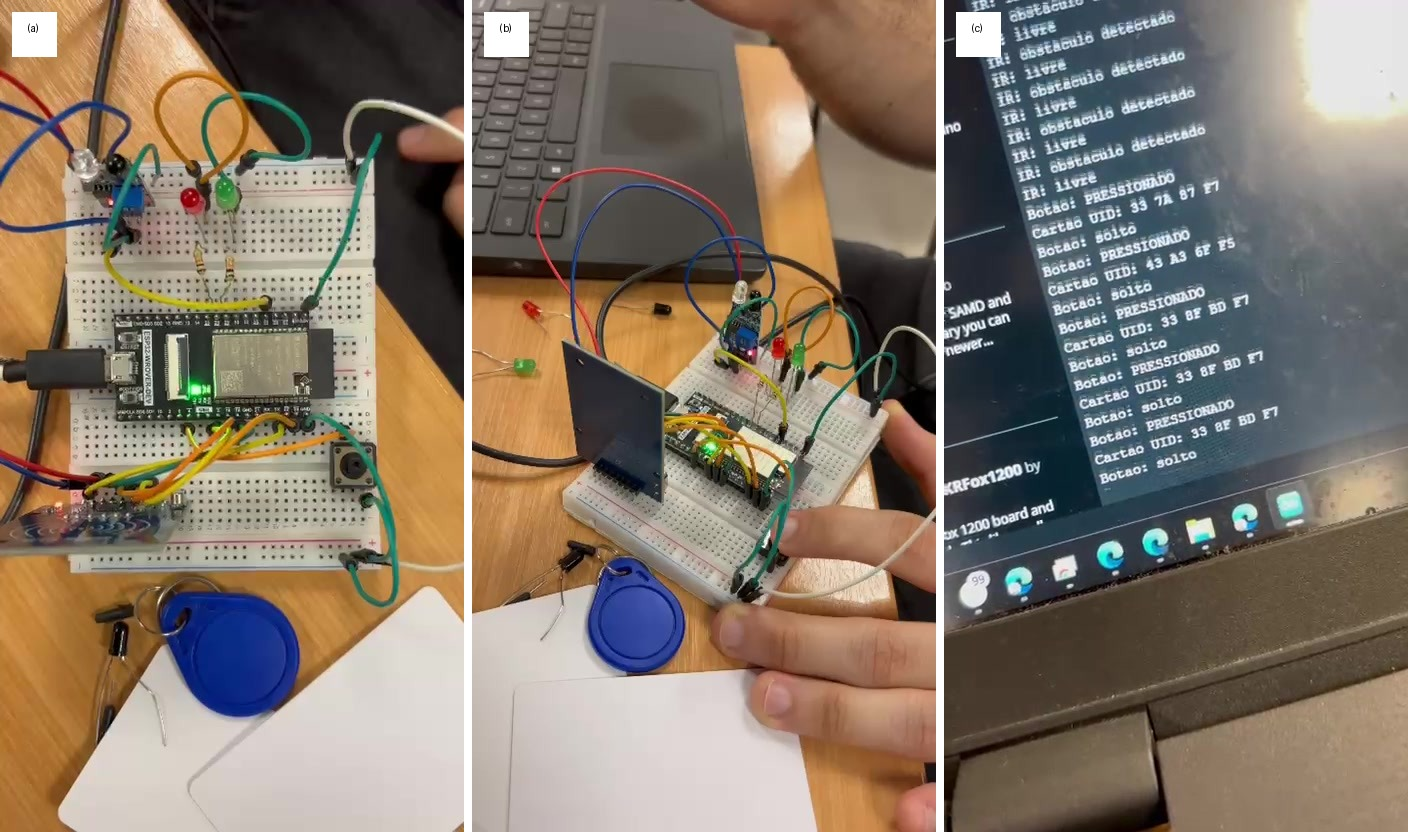
\includegraphics[width=\columnwidth]{prototipo.jpg}
\caption{Protótipo em funcionamento: (a) montagem em protoboard com
ESP32-WROVER, leitor RC522, sensor IR de obstáculo, botão e LEDs; (b) leitura
de uma tag RFID; (c) Monitor Serial registrando eventos do sensor IR, do botão
e os UIDs lidos.}
\label{fig:prototipo}
\end{figure}

A Tabela~\ref{tab:comparacao} compara os programas em Tupã com o C++ gerado e,
para o teste de hardware, com o C++ que seria escrito à mão
(\texttt{teste\_hardware.ino}, a referência). O controle de acesso passou de 12
para 100 linhas de código, cerca de 8,3 vezes mais, e o teste de hardware de 23
para 112, cerca de 4,9 vezes. O gerado tem cerca de 2,2 vezes as linhas do
manual (112 contra 51), porque inclui \textit{debounce} por \texttt{millis()}
com detecção de borda, espera de 3~s no NFC, encerramento do cartão, conferência
da lista de UIDs e funções auxiliares de LED, que o firmware manual não tem.
Nenhuma linha de configuração do hardware precisa ser escrita pelo usuário.

\begin{table}[htbp]
\caption{Tupã versus C++ gerado e C++ manual}
\begin{center}
\setlength{\tabcolsep}{3pt}
\begin{tabular}{lccccc}
\toprule
 & \multicolumn{2}{c}{\textbf{controle\_nfc}} & \multicolumn{3}{c}{\textbf{teste\_hardware}} \\
\cmidrule(lr){2-3}\cmidrule(lr){4-6}
\textbf{Métrica} & \textbf{Tupã} & \textbf{Gerado} & \textbf{Tupã} & \textbf{Gerado} & \textbf{Manual} \\
\midrule
Linhas totais             & 17 & 126 & 33 & 139 & 67 \\
Linhas de código          & 12 & 100 & 23 & 112 & 51 \\
Inclusões de bibliotecas  & 0  & 2   & 0  & 2   & 2  \\
Constantes (\texttt{\#define}) & 0 & 7 & 0 & 7 & 6 \\
Razão C++/Tupã            & \multicolumn{2}{c}{8,3} & \multicolumn{3}{c}{4,9} \\
\bottomrule
\end{tabular}
\label{tab:comparacao}
\end{center}
\end{table}

Linhas de código excluem linhas vazias e comentários. As duas inclusões são
\texttt{SPI.h} e \texttt{MFRC522.h}. Nos arquivos gerados, as sete constantes
são os pinos (cinco no \texttt{controle\_nfc}, seis no \texttt{teste\_hardware}),
a janela de \textit{debounce} e, no \texttt{controle\_nfc}, o \textit{timeout} do NFC. No manual, as seis constantes são pinos. Há uma diferença
conhecida de comportamento: o firmware manual mantém o LED vermelho aceso
enquanto o botão está apertado, e o programa em Tupã o acende por 300~ms a cada
aperto.

% TODO: tempo de compilação e de gravação na placa (medir com arduino-cli).
% TODO: testes com usuários, se houver.

% ===============================================================
\section{Conclusão e Trabalhos Futuros}\label{sec:conclusao}
% ===============================================================
Este artigo apresentou o Tupã, uma linguagem de domínio específico em
português para programação de microcontroladores ESP32, e seu compilador,
que percorre as quatro fases clássicas de compilação e gera C++ compatível
com o ecossistema Arduino. Os resultados preliminares indicam que a
linguagem reduz significativamente a quantidade de código que o usuário
precisa escrever e elimina a configuração manual do hardware, enquanto a
análise semântica orientada a módulos detecta erros antes da gravação. O
protótipo com ESP32-WROVER, RC522, sensor infravermelho de obstáculo, botão e
LEDs foi validado em bancada com um firmware escrito à mão, e os programas
gerados compilam com a Arduino CLI para a placa-alvo. Falta, porém, gravar o
\texttt{.ino} gerado na placa e repetir o teste de bancada com ele, de modo que
o funcionamento do código gerado no hardware ainda não foi verificado.

Os próximos passos incluem: gravar na placa o código gerado por
\texttt{controle\_nfc.tupa} e \texttt{teste\_hardware.tupa} e comparar seu
comportamento com o do firmware manual; automatizar a compilação e a gravação a
partir do comando \texttt{tupa build}; ampliar os módulos suportados, como o
envio de infravermelho, hoje fora do escopo; documentar a linguagem e o
compilador no repositório Git; e, fora do escopo do MVP, permitir a
atualização do firmware por Wi-Fi (OTA). Também se pretende avaliar o uso da
linguagem em contexto de ensino de sistemas embarcados.

\section*{Agradecimentos}
Os autores agradecem ao professor da disciplina de Linguagens Formais e
Compiladores do IBMEC pela orientação. % TODO: nome do professor (so o Joao sabe)

% ---------------------------------------------------------------
% Referências
% Referencias: anos e paginas conferidos de memoria, URLs NAO testadas online; ver lista de pendencias.
% ---------------------------------------------------------------
\begin{thebibliography}{00}
\bibitem{aho} A. V. Aho, M. S. Lam, R. Sethi, and J. D. Ullman, \textit{Compilers: Principles, Techniques, and Tools}, 2nd ed. Boston, MA: Addison-Wesley, 2006.
\bibitem{arduino} Arduino, ``Arduino language reference.'' [Online]. Available: \url{https://docs.arduino.cc/language-reference/}. Acesso em: nov. 2026.
\bibitem{arduinocli} Arduino, ``Arduino CLI.'' [Online]. Available: \url{https://arduino.github.io/arduino-cli/}. Acesso em: nov. 2026.
\bibitem{makecode} J. Devine, J. Finney, P. de Halleux, M. Moskal, T. Ball, and S. Hodges, ``MakeCode and CODAL: intuitive and efficient embedded systems programming for education,'' \textit{J. Syst. Archit.}, vol. 98, pp. 468--483, 2019.
\bibitem{blockly} N. Fraser, ``Ten things we've learned from Blockly,'' in \textit{Proc. IEEE Blocks and Beyond Workshop}, 2015, pp. 49--50.
\bibitem{flipper} Flipper Devices, ``Flipper Zero.'' [Online]. Available: \url{https://flipperzero.one/}. Acesso em: nov. 2026.
\bibitem{portugol} L. H. Noschang, A. Pelz, E. A. Raabe, and A. L. A. Raabe, ``Portugol Studio: uma IDE para iniciantes em programação,'' in \textit{Anais do Workshop sobre Educação em Computação (WEI/CSBC)}, 2014.
\bibitem{esp32} Espressif Systems, ``ESP32 series datasheet.'' [Online]. Available: \url{https://www.espressif.com/en/support/documents/technical-documents}. Acesso em: nov. 2026.
\bibitem{mfrc522} NXP Semiconductors, ``MFRC522: standard performance MIFARE and NTAG frontend,'' product data sheet. % TODO: ano/revisao e URL do datasheet
\end{thebibliography}

\end{document}